% Semiconductor pn junction diagram
% Author: Erwann Fourmond
\documentclass[tikz]{standalone}
%%%<
\usepackage{verbatim}
%%%>
\begin{comment}
:Title: Semiconductor pn junction diagram
:Tags: Decorations;Foreach;Diagrams;Physics
:Author: Erwann Fourmond
:Slug: junction-diagram

The junction here is drawn with photon injection condition
like in a solar cell, so we use the quasi-fermi levels.
\end{comment}
\usepackage{tikz}
\usetikzlibrary{patterns,arrows,calc,decorations.pathmorphing}

% Modified \textcircled macro
\renewcommand*\textcircled[1]{\tikz[baseline=(char.base)]{
  \node [shape=circle,draw,inner sep=1pt] (char) {#1};}}

\begin{document}
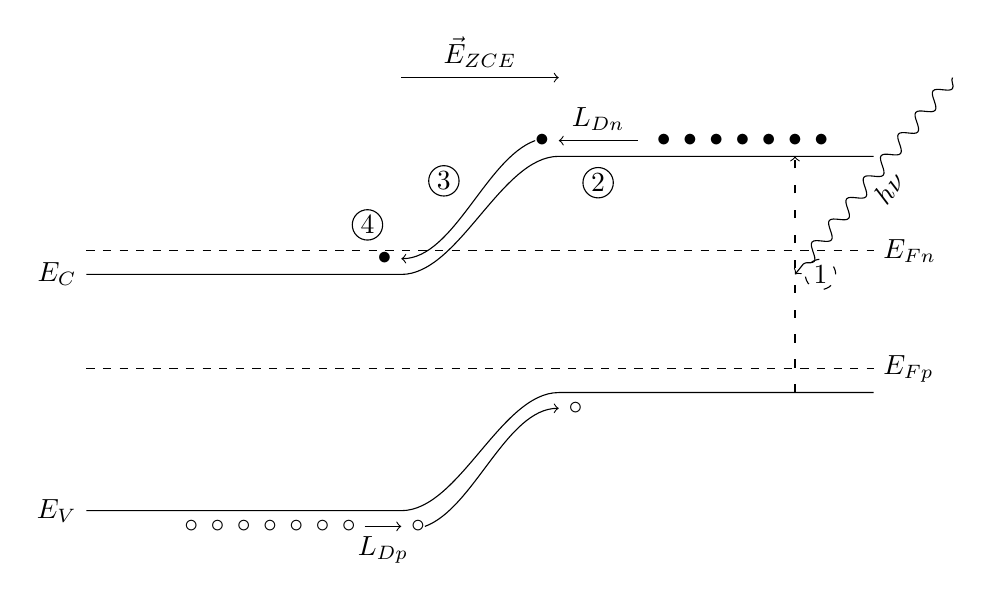
\begin{tikzpicture}
    % variables for pn-junction diagram:
    % all parameters are in tikz scale
    % p-side of the junction is here on the right

	\def\V{1.5}   % junction polarisation (0=flat band)
	\def\EG{3}    % band gap of semiconductor
	\def\EF{1.5}  % vertical Fermi level position
	\def\EFn{3.3} % pseudo fermi level for electrons
	\def\EFp{1.8} % pseudo fermi level for holes
	\def\DZCE{4}  % start position on the left for space charge region (SCR)
	\def\LZCE{2}  % SCR width
	\def\PN{10}   % total lentgh of the junction

  % calculations
  \pgfmathsetmacro\EC{\EG+\V};% conduction band heigth (without polarisation)
  \pgfmathsetmacro\FZCE{\DZCE+\LZCE};% SCR end position

  % valence and conduction band drawing: 
  \draw (0,0) node [left]{$E_V$} -- (\DZCE,0)
    to[out=0, in=180, looseness=0.75] (\FZCE,\V) -- (\PN,\V); % EV
  \draw (0,\EG) node [left] {$E_C$} -- (\DZCE,\EG)
    to[out=0, in=180, looseness=0.75] (\FZCE,\EC) -- (\PN,\EC); % EC

  % fermi level drawing (if needed):		
  %	\draw [dashed](0,\EF) -- ({\PN-0.5},\EF) node [right]{$E_F$}; % EF

  % quasi fermi levels drawing (if needed) :	
  \draw [dashed] (0,\EFn)  -- (\PN,\EFn)
    node [right] {$E_{Fn}$}; % EFn for electron
  \draw [dashed] (0,\EFp)  -- ({\PN},\EFp)
    node [right] {$E_{Fp}$}; % EFp for holes

  % electric field in SCR drawing :
  \draw [->] (\DZCE, {\V+\EG+1}) --
    node [above] {$\vec{E}_{ZCE}$} (\FZCE, {\V+\EG+1}) ; % E vector

  % excess carriers
  \foreach \x in {1,2,...,7}
    \draw ({\FZCE+1+\x/3},{\EC+0.2}) node {$\bullet$}; % p side : electrons
  \foreach \x in {1,2,...,7}
    \draw ({1+\x/3},{-0.2}) node {$\circ$}; % n side : holes

  % photon injection and carrier generation
  % p side : carrier generation:
  \draw [->, loosely dashed] ({\FZCE+3}, \V) --
    node [right] {\textcircled{1}}({\FZCE+3}, \EC);
  % the textcircled{number} option is used in several places
  % to describe the physical mechanisms.
  % It can be safely removed if not needed
  % photon wave injection in the bandgap on p-side :
  \draw [decorate, decoration={snake}, ->] ({\PN+1},{\EC+1}) --
    node [below,sloped]{$h\nu$} ({\FZCE+3}, \EG); 
		
  % excess carriers diffusion, with diffusion length :
  % electrons on p side :
  \draw [->] ({\FZCE+1},{\EC+0.2}) -- node [above] {$L_{Dn}$}
    node [below=6pt] {\textcircled{2}}({\FZCE},{\EC+0.2})
    node [left] {$\bullet$} ;
  \draw [->] ({\FZCE-0.3},{\EC+0.2}) to [out=200, in=0, looseness=0.75]
    node [above left] {\textcircled{3}} ({\DZCE},{\EG+0.2})
    node [left] {$\bullet$} node [above left=3pt] {\textcircled{4}};
  % holes on n side :
  \draw [->] ({1.2+7/3},{-0.2}) -- node [below] {$L_{Dp}$} ({\DZCE},{-0.2})
    node [right]{$\circ$} ;
  \draw [->] ({\DZCE+0.3},-0.2) to [out=20, in=180, looseness=0.75]
    ({\FZCE},{\V-0.2}) node [right]{$\circ$};
\end{tikzpicture}
\end{document}
